% Draft for IEEE Transactions on Signal Processing.
% Compiles with IEEEtran when it is installed. The fallback below only lets the draft build without it.
\IfFileExists{IEEEtran.cls}
  {\documentclass[journal]{IEEEtran}}
  {\documentclass[10pt,twocolumn]{article}\usepackage[margin=0.75in]{geometry}
   \newenvironment{IEEEkeywords}{\par\smallskip\noindent\textit{Index Terms:}\ }{\par}
   \newcommand{\IEEEPARstart}[2]{##1##2}
   \newcommand{\appendices}{\appendix}}
\usepackage{amsmath,amssymb,amsthm,booktabs,cite,graphicx}
\newtheorem{lemma}{Lemma}
\newtheorem{theorem}{Theorem}
\newtheorem{proposition}{Proposition}
\theoremstyle{remark}
\newtheorem{remark}{Remark}
\newcommand{\todo}[1]{\textit{[To be completed: #1]}}
\newcommand{\R}{\mathbb{R}}
\newcommand{\Z}{\mathbb{Z}}
\newcommand{\E}{\mathbb{E}}
\newcommand{\ip}[2]{\langle #1,#2\rangle}

\begin{document}
\title{Event Streams of Moving Scenes: Rate Limits and Regeneration Under Affine Motion}
\author{[Author list to be set]}
\maketitle

\begin{abstract}
An event camera reports the changes of each pixel's log intensity as asynchronous threshold
crossings. When a scene moves across the sensor, every pixel on the path of an edge observes the
same intensity profile, so the stream appears to describe that profile many times. It does not
repeat exactly: each pixel fires on its own lattice of threshold levels, whose offset, the
threshold phase, differs from pixel to pixel, and every event carries timing jitter. We determine
what these differences cost a code, for a ramp edge under an affine flow. Losslessly, the phase of
each pixel and the jitter of its other events must be described however well the scene and its
motion are known, so the rate per event does not fall with the length of the path. Under a mean-squared timing
tolerance there are three regimes. Below the jitter variance the code describes every event time.
Above it the code describes one number per pixel. Beyond a threshold set by the event spacing of
the pixel it describes nothing, because the events can be regenerated from the edge and its motion,
and what remains is the motion, at a cost that grows at most logarithmically with the path. The
rate-distortion function is exact in the first regime and known within $0.255$ bit per pixel in the
second. These results lead to a codec that transmits the events of one window as a template and one
affine map for each later window, and we quantify what moving events loses against regenerating
them.
% PROVISIONAL (verify against the final experiments before submission): the next sentence states
% what directives 001 to 005 measured with annotated regions and without the bits of the regions.
On traffic recordings, a motion-compensated template shortens the lossless code only
slightly, the fidelity of regenerated events at a fixed tolerance rises with object speed, and
regeneration reaches a given fidelity with a fraction of the events that random thinning needs.
\end{abstract}

\begin{IEEEkeywords}
Event camera, send-on-delta sampling, level-crossing sampling, rate-distortion theory, generalized
sampling, motion compensation, neuromorphic sensing.
\end{IEEEkeywords}

\section{Introduction}
\IEEEPARstart{A}{n} event camera has no frames. Each pixel compares its log intensity with a stored
reference and emits an event, with a time stamp and a polarity, whenever the difference reaches a
contrast threshold \cite{lichtsteiner2008,gallego2022survey}. The output is a stream of
address-events whose rate follows the scene: it is close to zero for a static scene and rises with
the speed and the contrast of what moves. A sensor node that forwards this stream over a
rate-limited link must decide how many bits the stream needs.

The stream of a moving scene looks highly redundant. If an object moves across the sensor, the
pixels along the path of one of its edges observe the same intensity profile, one after the other.
Yet they do not emit the same events. Each pixel compares the intensity with its own reference, so
it fires on its own lattice of levels, and the offset of that lattice, the threshold phase of the
pixel, differs from pixel to pixel. The same profile therefore produces a different event train at
every pixel (Fig.~\ref{fig:mechanism}). This paper asks what these differences cost: how many bits
a code needs to preserve them, and how many it saves when a timing error is allowed.

The setting has precedents in sampling theory. An event pixel is a send-on-delta sampler
\cite{miskowicz2006}, which for a monotone input coincides with level-crossing sampling
\cite{mark1981,martineznuevo2019}. An object that crosses $M$ pixels is sampled by $M$ such
samplers, which recalls the generalized sampling expansion \cite{papoulis1977gse}, by which a
bandlimited signal is recovered from the outputs of $m$ linear systems that are each sampled at
$1/m$ of the Nyquist rate. In multi-channel time encoding, several integrate-and-fire encoders
with shifted integrators share one input, and the shifts are what make the channels complementary
\cite{lazar2004,adam2020multichannel,adam2022}. The threshold phases play that role here.

Existing event coders approach the rate empirically. Lossless coders exploit the spatial and temporal
correlation of addresses and time stamps \cite{bi2018,khan2021talven,schiopu2022spl}. Lossy coders
discard or aggregate events \cite{banerjee2021icip,huang2023icip}, and the coder of
\cite{stumpp2024} suppresses events that an on-sensor optical flow can predict and lets the receiver
extrapolate them. A recent survey notes that reported results are hard to compare
\cite{brites2025}, and no accepted distortion measure for lossy event coding exists
\cite{rezaee2026}. On the theoretical side, rate-distortion results for point processes concern
Poisson and finite point processes \cite{rubin1974,verdu1996,lapidoth2015,koliander2018}. They do
not model events that a moving profile generates through a threshold rule.

This paper models that mechanism and derives what a code can and cannot save. Its central result
is the rate-distortion function of the events of a pixel under a timing tolerance. The other
results lead to it or follow from it.

\emph{1) Mechanism.} Given the edge and its motion, the events of a pixel are a function of a
single number, its threshold phase, up to timing jitter. The phase is a property of the pixel and
is independent across pixels. Next to what the pixels of a path share, the edge and its motion,
each pixel therefore has something private. A lossless code must describe it for every pixel, and
its rate per event does not decrease with the number $M$ of pixels on the path
(Theorem~\ref{thm:lossless}).

\emph{2) Rate under a timing tolerance.} The tolerance decides which of the private quantities a
code must describe (Theorem~\ref{thm:pixel}). Below the jitter variance it describes all of them,
and the rate is known exactly. Above it one number per pixel remains, and the rate is known within
$0.255$ bit. Beyond a threshold that grows with the event spacing of the pixel, the contrast
threshold divided by the rate of change of its intensity, the rate is zero: the decoder regenerates
the events from the edge and its motion. Slowly crossed pixels need a larger tolerance. Along a
path, a description of the motion of $O(\ln M)$ nats then replaces a lossless description of order
$M$.

\emph{3) Regeneration in practice.} A sender has the events and not the edge. We replace the edge
by the events of a key window, which the receiver moves along a fitted affine map. Moved events
keep the phases of the pixels they came from, and we show that this doubles the timing error of the
ideal decoder at equal event spacings (Proposition~\ref{prop:moved}). We measure the codec in total
bits on traffic recordings \cite{verma2024etram}. \todo{one sentence on the second dataset
\cite{gehrig2021dsec} once it has been measured.}

Section~\ref{sec:model} states the model. Sections~\ref{sec:lossless} and~\ref{sec:tolerance}
contain the theory. Section~\ref{sec:codec} describes the codec, and Section~\ref{sec:experiments}
the measurements. Proofs are in the appendices. Rates are in nats unless bits are named, $\|\cdot\|$
is the Euclidean norm of a vector and the spectral norm of a matrix, and $[x]^+=\max(x,0)$.

\section{Model}\label{sec:model}
We first state the pixel rule, from which the phase mechanism follows for any scene. We then
specialize to a ramp edge in uniform passage, for which the rates have closed forms.
\subsection{Pixel}
Pixels sit at the lattice points $i\in\Z^2$ of the image plane. Pixel $i$ observes the log intensity
$\ell_i(t)=L(i,t)$ of a continuous field $L$.

\textbf{(A1) Send-on-delta.} Pixel $i$ holds a reference $\mu_i$ with $|\ell_i-\mu_i|<C$ at the
start. It emits an event at the first time $t$ at which $|\ell_i(t)-\mu_i|=C$, with polarity
$p=\operatorname{sign}(\ell_i(t)-\mu_i)$, and then sets $\mu_i\leftarrow\mu_i+pC$. The contrast
threshold $C>0$ is common to all pixels and known to the decoder. The \emph{phase} of the pixel is
the number $a_i\in(0,C]$ with $\mu_i\in a_i+C\Z$ at the start.

\subsection{Scene and Motion}
A template $g:\R^2\to\R$ gives the log intensity in object coordinates. At time $t$ the object
point $u$ is at the image position $\phi_t(u)=J_tu+b_t$, with $J_t\in\R^{2\times2}$ invertible, so
\begin{equation}\label{eq:field}
  L(x,t)=g\big(\phi_t^{-1}(x)\big)
\end{equation}
and pixel $i$ observes
\begin{equation}\label{eq:traj}
  \ell_i(t)=g\big(u_i(t)\big),\qquad u_i(t)=J_t^{-1}(i-b_t).
\end{equation}
The curve $u_i$ is the trajectory of pixel $i$ in object coordinates. The velocity field
$v(x,t)=\dot\phi_t(\phi_t^{-1}(x))$ is affine in $x$ and satisfies the brightness constancy
relation
\begin{equation}\label{eq:constancy}
  \frac{\partial L}{\partial t}(x,t)+\ip{\nabla L(x,t)}{v(x,t)}=0,
\end{equation}
which follows from differentiating $L(\phi_t(u),t)=g(u)$ in $t$. We call the motion an
\emph{affine flow} when the velocity field is also constant in time,
\begin{equation}\label{eq:flow}
  v(x)=\Lambda x+v_0,
\end{equation}
with generator $\Lambda\in\R^{2\times2}$. A translation has $\Lambda=0$. The trace of $\Lambda$ is
the rate at which the object grows or shrinks in area, its antisymmetric part rotates the object,
and its symmetric traceless part shears it. At a given instant, any smooth velocity field has the
form \eqref{eq:flow} to first order in $x$ around a point, so \eqref{eq:flow} is the local model of
a general motion over a short time.

\subsection{Edge}
\textbf{(A2) Ramp edge.} The template is a ramp across a line with unit normal $\nu$,
\begin{equation}\label{eq:ramp}
  g(u)=\varrho\big(\ip{\nu}{u}-c_0\big),\qquad
  \varrho(z)=\begin{cases}0,&z\le0,\\ \gamma z,&0\le z\le w,\\ V,&z\ge w,\end{cases}
\end{equation}
with slope $\gamma>0$, width $w$ and height $V=\gamma w=nC$ for an integer $n\ge1$.

Pixel $i$ sees the edge through its edge coordinate
\begin{equation}\label{eq:z}
  z_i(t)=\ip{\nu}{u_i(t)}-c_0,\qquad \ell_i(t)=\varrho\big(z_i(t)\big).
\end{equation}
\textbf{(A2$'$) Uniform single passage.} The edge passes pixel $i$ once: $z_i<0$ before a time
$t_i$, $z_i>w$ after the passage, and in between $z_i$ is affine in $t$ with slope $r_i>0$.

Inside the ramp, $\nabla L=\gamma\nu_t$ with $\nu_t=J_t^{-\top}\nu$ a normal of the edge in the
image, and $\dot z_i=-\ip{\nu_t}{v(i,t)}$. By \eqref{eq:constancy}, the intensity of pixel $i$
rises during the passage at the rate
\begin{equation}\label{eq:rate}
  \gamma r_i=-\ip{\nabla L}{v}=\|\nabla L\|\,v_{\perp,i},
\end{equation}
with the field evaluated at pixel $i$. Here $v_{\perp,i}=-\ip{\nabla L}{v}/\|\nabla L\|$ is the
speed at which the edge advances over the pixel along its normal, counted positive when the
intensity of the pixel rises, as it does in a passage with $r_i>0$. We call
\begin{equation}\label{eq:tau}
  \tau_i=\frac{C}{\gamma r_i}=\frac{C}{\|\nabla L\|\,v_{\perp,i}}
\end{equation}
the \emph{event spacing} of pixel $i$. It is the time that the ramp takes to pass the pixel,
divided by $n$. At a fixed image slope $\|\nabla L\|$ it is inversely proportional to the normal
speed of the edge. Assumption (A2$'$) holds exactly for a translation, where $\tau_i$ is the same
for all pixels, and for a plane that approaches the camera along the optical axis at constant
speed, where $J_t^{-1}$ is affine in $t$ and $b_t$ is fixed. For an affine flow it holds to first
order (Remark~\ref{rem:passage}), and $\tau_i$ varies from pixel to pixel.

\subsection{Phase, Jitter and Clock}
\textbf{(A3) Phase.} Before the edge arrives, pixel $i$ rests at the level $0$ with its reference
behind the passage, $\mu_i\in(-C,0]$, so that $a_i=\mu_i+C$. The phases $a_i$ are independent
across pixels, uniform on $(0,C]$, and independent of the jitter.

\textbf{(A4) Jitter and clock.} The $k$th event of pixel $i$ is recorded at
$T_{i,k}=t_{i,k}+\varepsilon_{i,k}$, where $t_{i,k}$ is the time given by (A1) and the
$\varepsilon_{i,k}$ are independent $\mathcal N(0,\sigma^2)$ variables, independent of the phases,
with $\sigma>0$. The stored value is $Y_{i,k}=\delta\lfloor T_{i,k}/\delta\rfloor$ for a clock
resolution $\delta$. The index $k$ of each recorded event is known.

The uniform phase does not arise inside the model, in which every pixel rests at the same level. It
stands for the offsets of real pixels and for their earlier activity. A pixel that the edge crosses
from the high level to the low level is covered by the mirrored assumption, with its reference in
$[V,V+C)$. Remark~\ref{rem:relax} treats a reference that is ahead of the passage.

We write $T_i=(T_{i,1},\dots,T_{i,n})$ and $Y_i=(Y_{i,1},\dots,Y_{i,n})$, and $\mathcal P$ for the
set of pixels that the edge passes during the observation, with $M=|\mathcal P|$. Let
$\eta(a,\sigma)$ denote the differential entropy of the sum of a uniform variable on $(0,a)$ and an
independent $\mathcal N(0,\sigma^2)$ variable. It satisfies
\begin{equation}\label{eq:eta}
  \tfrac12\ln\!\big(a^2+2\pi e\sigma^2\big)\le\eta(a,\sigma)\le\tfrac12\ln\!\big(2\pi e(a^2/12+\sigma^2)\big)
\end{equation}
by the entropy power inequality \cite[Ch.~17]{cover2006elements} and by the Gaussian bound on the
entropy at a given variance \cite[Ch.~8]{cover2006elements}, and $\eta(a,\sigma)-\ln a\to0$ as
$\sigma/a\to0$.

\section{Structure and Lossless Limit}\label{sec:lossless}
\begin{lemma}\label{lem:lattice}
Under (A1), for any continuous $\ell_i$, every event of pixel $i$ occurs at a time $t$ with
$\ell_i(t)\in a_i+C\Z$.
\end{lemma}
The lattice $a_i+C\Z$ never changes. The phase is a property of the pixel, set by its history and
not by the edge that passes.
\begin{lemma}\label{lem:times}
Under (A1), (A2), (A2$'$) and $\mu_i\in(-C,0]$ before the passage, pixel $i$ emits exactly $n$
events, all of positive polarity, at
\begin{equation}\label{eq:times}
  t_{i,k}=t_i+A_i+(k-1)\tau_i,\qquad k=1,\dots,n,
\end{equation}
where $A_i=a_i/(\gamma r_i)$. Under (A3), $A_i$ is uniform on $(0,\tau_i]$.
\end{lemma}
\begin{figure}[t]
\centering
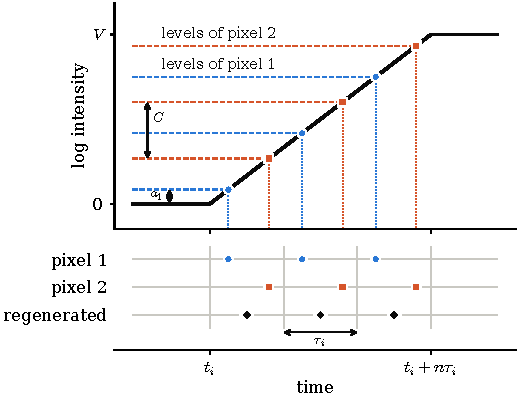
\includegraphics[width=\columnwidth]{figs/fig_mechanism.pdf}
\caption{One ramp, two pixels with different threshold phases, and the regenerated events
\eqref{eq:regen}. Time is measured from the arrival of the edge at each pixel. Jitter is omitted.}
\label{fig:mechanism}
\end{figure}
Given the template and the flow, the noise-free events of a pixel are thus a function of one
number, its phase. Fig.~\ref{fig:mechanism} shows two pixels with $n=3$ that see the same ramp: the
intensity trajectories coincide, and the event trains differ by the difference of the phases. In the object coordinate, an event is a point of the graph of the profile on the
level lattice of its pixel: the $M$ pixels of a path sample the same profile on $M$ lattices with
independent offsets.
\begin{theorem}[Lossless code length]\label{thm:lossless}
Under (A1) to (A4) and (A2$'$), the vectors $T_i$, $i\in\mathcal P$, are independent given the
template and the flow,
\begin{equation}\label{eq:hT}
  h(T_i)=\frac{n-1}{2}\ln(2\pi e\sigma^2)+\eta(\sqrt n\,\tau_i,\sigma),
\end{equation}
and
\begin{equation}\label{eq:HY}
  H(Y_i\mid g,\phi)=n\ln\frac1\delta+h(T_i)+e_\delta,
\end{equation}
where $e_\delta\ge0$ for every $\delta$, and $e_\delta\to0$ as $\delta/\sigma\to0$, uniformly in
$\tau_i$.
\end{theorem}
When $\sigma\ll\tau_i$ and $\delta\ll\sigma$, \eqref{eq:HY} gives the cost per event
\begin{equation}\label{eq:perevent}
  \frac{H(Y_i\mid g,\phi)}{n}\approx\frac{n-1}{n}\ln\frac{\sigma\sqrt{2\pi e}}{\delta}
  +\frac1n\ln\frac{\sqrt n\,\tau_i}{\delta}.
\end{equation}
One event of each pixel pays for the phase and the other $n-1$ pay for jitter. The code length of
the path is the sum of \eqref{eq:HY} over $\mathcal P$. It grows in proportion to $M$, and neither
term of \eqref{eq:perevent} falls as the path gets longer: a decoder that knows the edge and its
motion exactly still pays \eqref{eq:perevent} for every event. What the pixels of a path share,
the edge and its motion, a code can describe once. What is private to each pixel, its phase and its
jitter, it must describe for each pixel, and \eqref{eq:HY} is that irreducible conditional rate.
Section~\ref{sec:experiments} measures how much more a code pays that does not know the motion.

\begin{remark}[Accuracy of the uniform passage]\label{rem:passage}
For an affine flow \eqref{eq:flow}, $\dot\nu_t=-\Lambda^{\!\top}\nu_t$ and
$\ddot z_i=\ip{\nu_t}{\Lambda v(i)}$, hence $|\ddot z_i|\le\kappa_i|\dot z_i|$ with
$\kappa_i=\|\Lambda\|/|\cos\vartheta_i|$, where $\vartheta_i$ is the angle between the velocity
$v(i)$ and the normal $\nu_t$. Take $r_i$ as the slope of $z_i$ at $t_i$. Over a passage of
duration $P_i=n\tau_i$, the event times then deviate from \eqref{eq:times} by at most
$\kappa_iP_i^2/2$, to first order in $\kappa_iP_i$. For a generator of norm $0.3\,\mathrm{s}^{-1}$,
a passage of $5$~ms and motion along the normal this is $4\,\mu$s, three orders of magnitude below
the passage time. The bound grows without limit for edges that are nearly parallel to their motion.
Such edges pass few pixels per unit time and contribute few events.
\end{remark}
\begin{remark}[Several edges]\label{rem:texture}
Theorem~\ref{thm:lossless} counts one edge that passes each pixel once. If further edges of the
same object pass the same pixel, they meet the same lattice, so the phase is paid once per pixel and
not once per edge. With many edges per pixel the cost per event tends to the jitter term
$\ln(\sigma\sqrt{2\pi e}/\delta)$, which does not depend on the path either.
\end{remark}

\section{Rate Under a Timing Tolerance}\label{sec:tolerance}
The encoder and the decoder know the template and the flow. The decoder outputs
$\hat T_i\in\R^n$ for each pixel, and the distortion is the mean-squared timing error
\begin{equation}\label{eq:dist}
  d(T_i,\hat T_i)=\frac1n\|T_i-\hat T_i\|^2 .
\end{equation}
\subsection{One Pixel}
Let $R_i(D)=\inf I(T_i;\hat T_i)$, with the infimum over the conditional laws of $\hat T_i$ that
satisfy $\E\,d(T_i,\hat T_i)\le D$, be the rate-distortion function of the events of pixel $i$. It
is the rate that block codes over many independent passages approach. Define
\begin{equation}\label{eq:defs}
  s_i^2=\frac{n\tau_i^2}{12}+\sigma^2,\qquad D_{A,i}=\sigma^2+\frac{\tau_i^2}{12},
\end{equation}
\begin{equation}\label{eq:gap}
  \Gamma_i=\tfrac12\ln(2\pi e\,s_i^2)-\eta(\sqrt n\,\tau_i,\sigma).
\end{equation}
By \eqref{eq:eta}, $0\le\Gamma_i\le\tfrac12\ln(2\pi e/12)$, which is $0.255$ bit, for every
$\sigma$ and $\tau_i$.
\begin{theorem}[Rate-distortion function of a pixel]\label{thm:pixel}
Under (A1) to (A4) and (A2$'$),
\begin{equation}\label{eq:rdlow}
  R_i(D)=h(T_i)-\frac n2\ln(2\pi eD)\qquad\text{for }0<D\le\sigma^2,
\end{equation}
\begin{equation}\label{eq:rdmid}
  \big[U_i(D)-\Gamma_i\big]^+\le R_i(D)\le U_i(D)\qquad\text{for }\sigma^2<D<D_{A,i},
\end{equation}
\begin{equation}\label{eq:rdzero}
  R_i(D)=0\qquad\text{for }D\ge D_{A,i},
\end{equation}
with
\begin{equation}\label{eq:U}
  U_i(D)=\frac12\ln\frac{s_i^2}{nD-(n-1)\sigma^2}.
\end{equation}
Moreover,
\begin{equation}\label{eq:rdpos}
  R_i(D)\ge\frac{n\,(D_{A,i}-D)}{2s_i^2}\qquad\text{for }0<D\le D_{A,i},
\end{equation}
so that $R_i(D)>0$ for $D<D_{A,i}$.
\end{theorem}
The three regimes have a direct reading. Below the jitter variance, every bit of timing precision
costs a bit, per event: the rate falls by $\log_210=3.32$ bits per event and per decade of the
root-mean-square tolerance $\sqrt D$. Between $\sigma^2$ and $D_{A,i}$, the $n-1$ jitter components
orthogonal to a common shift of the events are no longer described, and the code describes one
number per pixel, the phase together with the mean jitter, to within $0.255$ bit. From $D_{A,i}$
on, nothing is described. The decoder that attains \eqref{eq:rdzero} outputs the mean times
\begin{equation}\label{eq:regen}
  \hat T_{i,k}=t_i+\big(k-\tfrac12\big)\tau_i,\qquad k=1,\dots,n .
\end{equation}
It \emph{regenerates} the events of the pixel from the edge and the flow. Each regenerated event is
within $\tau_i/2$ of its noise-free time, and the count and the polarities are exact.

Two of these statements extend beyond the ramp. If the noise-free event times of a pixel are any
function of its phase, \eqref{eq:rdlow} holds below the jitter variance with the entropy of the
actual event times, and the smallest distortion at zero rate is
$\tfrac1n\operatorname{tr}\operatorname{Cov}(T_i)$, attained by the mean times. The middle regime,
in which one number per pixel is described to within $0.255$ bit, and the closed forms
\eqref{eq:hT}, \eqref{eq:U} and \eqref{eq:defs} belong to the ramp in uniform passage, where the
phase shifts all events of a pixel by a common time.

The threshold $D_{A,i}$ grows with the square of the event spacing. By \eqref{eq:tau}, a pixel whose
intensity changes slowly has a large spacing and needs a large tolerance before its events can be
regenerated, and a pixel that is crossed quickly needs a small one.

\subsection{A Path}
For the $M$ pixels of a path, let the distortion be the average of \eqref{eq:dist} over
$i\in\mathcal P$, and let $R_{\mathcal P}(D)$ be the rate-distortion function of
$(T_i)_{i\in\mathcal P}$ under it.
\begin{theorem}[Rate-distortion function of a path]\label{thm:path}
Under (A1) to (A4) and (A2$'$),
\begin{equation}\label{eq:alloc}
  R_{\mathcal P}(D)=\min\Big\{\sum_{i\in\mathcal P}R_i(D_i):\ \frac1M\sum_{i\in\mathcal P}D_i\le D\Big\}.
\end{equation}
In particular,
\begin{equation}\label{eq:pathlow}
  R_{\mathcal P}(D)=\sum_{i\in\mathcal P}h(T_i)-\frac{Mn}{2}\ln(2\pi eD)\qquad\text{for }0<D\le\sigma^2,
\end{equation}
and $R_{\mathcal P}(D)=0$ if and only if
\begin{equation}\label{eq:pathzero}
  D\ \ge\ \bar D_A=\sigma^2+\frac1{12M}\sum_{i\in\mathcal P}\tau_i^2 .
\end{equation}
If $\tau_i\le\tau_{\max}$ on the path, then for $D\le\bar D_A$
\begin{equation}\label{eq:pathpos}
  R_{\mathcal P}(D)\ge\frac{nM\,(\bar D_A-D)}{2\,(n\tau_{\max}^2/12+\sigma^2)} .
\end{equation}
\end{theorem}
If the tolerance is imposed on every pixel separately, the rate is zero if and only if
$D\ge\max_iD_{A,i}$, and the slowest crossing sets the tolerance. By \eqref{eq:pathpos}, below
$\bar D_A$ a rate that is proportional to $M$ remains.

\subsection{The Motion}
Theorems~\ref{thm:pixel} and~\ref{thm:path} assume that the decoder knows the flow. It remains to
count what describing the flow costs.
\begin{proposition}[Description of the motion]\label{prop:motion}
Let the flow depend on a parameter $\theta=(\theta_1,\dots,\theta_q)$ that ranges over a box whose
$j$th side has length at most $L_jM^{\alpha_j}$, and let the mean times
$\bar t_{i,k}(\theta)=t_i(\theta)+(k-\tfrac12)\tau_i(\theta)$ of \eqref{eq:regen} satisfy
$|\partial\bar t_{i,k}/\partial\theta_j|\le S_jM^{\beta_j}$ on the box, for all events of the path,
with constants $L_j,S_j>0$ and exponents $\alpha_j,\beta_j\ge0$ that do not depend on $M$. Then
for every $\xi>0$ the events of the path can be described with average distortion at most
$(1+\xi)\bar D_A$ using
\begin{equation}\label{eq:B}
  B\le\Big(\sum_{j=1}^q(\alpha_j+\beta_j)\Big)\ln M+O(1)\quad\text{nats,}
\end{equation}
where the $O(1)$ term depends on $q$, $\xi$, $\sigma$ and the constants and not on $M$.
\end{proposition}
For a translation along a line with a speed in a fixed interval that excludes zero, $\theta$ holds
the position of the edge, with a range of order $M$ and a sensitivity of order one, and the speed,
with a range of order one and a sensitivity of order $M$, so $B\le2\ln M+O(1)$. The same holds with
finite exponents, and hence $B=O(\ln M)$, for an affine flow whose normal speed is bounded away from
zero on the path and whose duration is polynomial in $M$. The lossless cost of the same events is
the sum of \eqref{eq:HY}, of order $M$, so the ratio of the two grows at least as $M/\ln M$. Above
$\bar D_A$ the description that remains is $O(\ln M)$. Below it, a rate proportional to $M$
remains. The bound \eqref{eq:B} is for a receiver that holds the edge. Section~\ref{sec:codec}
accounts for the template and the regions.

\begin{remark}[Event count under a change of scale]\label{rem:count}
An edge segment emits $n$ events for every pixel that it passes, so its event rate is $n$ times the
area that it sweeps per unit time, that is $n$ times its length times its mean normal speed. Under
a similarity flow about a fixed point, growth by a factor $\zeta$ makes the segment $\zeta$ times
longer and $\zeta$ times faster, and the rate grows as $\zeta^2$. For an object that approaches at
constant speed, the image speed itself grows as $\zeta^2$ and the rate as $\zeta^3$. A regeneration
that moves a fixed set of events keeps their number. Under a change of scale it must also change
the number of events, or regenerate them from the edge.
\end{remark}
\begin{remark}[Departures from the model]\label{rem:relax}
\emph{Reference ahead of the passage.} If $\mu_i\in(0,C)$ before a rising passage, as after a
passage of the opposite polarity at the same pixel, the first level that the intensity meets is the
reference itself, which does not fire. The pixel then emits $n-1$ events, and the results hold with
$n-1$ in place of $n$ and $t_i+\tau_i$ in place of $t_i$.
\emph{Height.} If the height of the edge is not a multiple of the threshold, $V/C=n+f$ with
$0<f<1$, pixel $i$ emits $n+1$ events when $a_i\le fC$ and $n$ otherwise. Reproducing the count
exactly costs the binary entropy of $f$ per pixel, and a zero-rate statement then holds only for a
distortion measure that tolerates one unmatched event per pixel, with a modified threshold.
\emph{Sensor.} Noise events, threshold mismatch between pixels, a refractory time and a jitter that
depends on the slope are outside the model, and their effect on the three regimes is not analyzed
here.
\end{remark}

\section{A Regenerating Codec}\label{sec:codec}
The decoder \eqref{eq:regen} needs the edge and the flow. A practical sender has neither. It has
the events. The codec of this section replaces the edge by events that the receiver already holds
and the flow by a map that the sender fits.

\subsection{Template, Motion and Groups}
Time is cut into windows of length $T_0$, and the windows of a region form groups of $K$. In the
first window of a group, the key window, the sender transmits the events of the region. For each of
the following $K-1$ windows it transmits one affine map. The receiver moves every key event
$(x,p,t)$ to the pixel nearest to the image of $x$ under the map and to the time $t+mT_0$, where
$m$ counts the windows since the key window, and it keeps the polarity. The moved events are its
reconstruction of window $m$. Under an affine flow, the map from one instant to an instant $mT_0$
later is the same for all instants of a window, so one map per window is exact for the positions
of the edges. It does not change the number of events, which a change of scale does
(Remark~\ref{rem:count}).

An affine map is described by six integers: a displacement in pixels, and four shape parameters
that give the displacement of the edges of the bounding rectangle of the key events, two for a
stretch along each axis and two for shear and rotation. With all shape parameters zero the map is a
translation.

The sender chooses the map of each window to maximize the fidelity \eqref{eq:fid} of the moved key
events against the true events of that window on one fixed working grid. Results on other grids
use the same maps. The search is coarse to fine, starts from the displacement predicted by the
velocity of the region, and never returns a map that is worse than the translation.

\subsection{Moved Events Against Regenerated Events}
The codec differs from the decoder \eqref{eq:regen} in three ways. It moves the phases of the key
pixels where \eqref{eq:regen} outputs the mean over the phase, it moves the jitter of the key
events, and it moves a fixed number of events. The first two have a price that the model gives
exactly.
\begin{proposition}[Moved events]\label{prop:moved}
Let the same edge pass pixel $j$ in the key window and a different pixel $i$ later, under (A1) to
(A4) and (A2$'$), and let the map be exact, so that the $k$th event of pixel $j$ is moved to pixel
$i$ at the time $\tilde T_{i,k}=T_{j,k}+t_i-t_j$. Then
\begin{equation}\label{eq:moved}
  \frac1n\,\E\|T_i-\tilde T_i\|^2=D_{A,i}+D_{A,j}+\frac{4n^2-1}{12}\,(\tau_i-\tau_j)^2 .
\end{equation}
\end{proposition}
With equal event spacings the error is $2D_A$, twice that of \eqref{eq:regen}: the codec trades a
factor of two in the timing error for not needing the edge. Unequal spacings, as under a change of
scale, add the last term, which grows with the square of the number of events per pixel. If the
moved events fall on their own pixel, as for an object that is nearly at rest, the phases coincide
and only the jitter term $2\sigma^2$ remains. The third difference, the number of events, is not a
timing error. It is measured in Section~\ref{sec:experiments}.

\subsection{Receiver Representation and Fidelity}
The theory uses the timing error \eqref{eq:dist}, which presupposes that regenerated and true
events are paired. For measured streams we use the representation that event-based receivers
compute, a voxel grid: the number of events of each polarity in blocks of
$\Delta_x\times\Delta_x$ pixels and in time bins of length $\Delta_t$. For a regenerated set with
voxel counts $c'$ and a true set with counts $c$, of sizes $N'$ and $N$, the fidelity is
\begin{equation}\label{eq:fid}
  F=\frac{2\sum\min(c',c)}{N'+N},
\end{equation}
the share of the events of the two sets that can be paired one to one inside a voxel. A subset
that holds a share $\chi$ of the events has $F=2\chi/(1+\chi)$ on every grid, whichever events it
keeps. For a codec that sends a share $\chi$ of the events of a group and reaches the fidelity $F$
over the group, the key window included, we report
\begin{equation}\label{eq:gain}
  G=\frac{F/(2-F)}{\chi},
\end{equation}
the factor by which it lowers the number of events sent at equal fidelity against thinning. The
factor counts events and serves as an explanation. The main results are in total bits, which
include the key events, the maps and the description of the regions.

The fidelity \eqref{eq:fid} and the timing error \eqref{eq:dist} are different distortion
measures, and the bin length plays the role of the tolerance. One case connects them. For blocks of
one pixel, a train that is long against the event spacing, and a jitter that is small against the
bin, Lemma~\ref{lem:times} gives the fidelity of the regenerated events \eqref{eq:regen} directly:
a bin holds at most one event of each train when $\Delta_t\le\tau_i$, the offset between the two
trains is uniform, and in expectation over the phase
\begin{equation}\label{eq:binfid}
  F=\frac{\Delta_t}{\tau_i}\qquad\text{for }\Delta_t\le\tau_i,
\end{equation}
with $F=1$ at $\Delta_t=\tau_i$. The voxel counts of a pixel are thus reproduced only when the bin
is at least as long as its event spacing, the same scaling as the threshold of
Theorem~\ref{thm:pixel}, for which $\sqrt{D_{A,i}}=\tau_i/\sqrt{12}$ when $\sigma\ll\tau_i$. In
larger blocks the independent phases of the pixels average, and the fidelity is higher at a given
bin length.

\todo{Regions. In the measurements so far a region is an annotated object. The paper needs regions
that the sender finds without annotation.}

\section{Experiments}\label{sec:experiments}
\todo{This section is an outline. It is organized by four questions, one figure each. The protocol
below is fixed before the simulations are run. Numbers appear only in this section.}

\subsection{Protocol}
\todo{(i) Controlled experiments use synthetic pixels under the model and the timing error
\eqref{eq:dist}. Recorded experiments use the voxel fidelity \eqref{eq:fid} and total bits.
(ii) One fixed working grid for fitting the maps. Other grids are evaluated with the same maps.
(iii) Baselines: thinning, whose fidelity is $2\chi/(1+\chi)$ by construction; repeating the key
events without motion; the translation alone; and coding all events after quantizing them to the
receiver grid.
(iv) Regions: annotated objects as the ideal case, and one automatic scheme, with the bits that
describe the regions counted.
(v) Main axis: total bits against fidelity.}

\subsection{The Three Regimes}
% Numbers and figure: directive 006, results/rd/regimes.json and results/rd/fig_regimes.pdf at f063a79.
\begin{figure}[t]
\centering
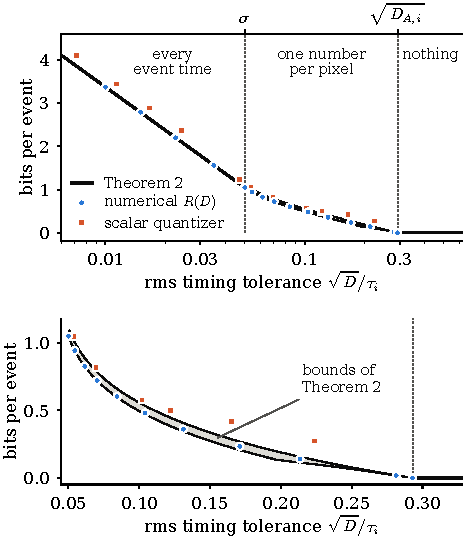
\includegraphics[width=\columnwidth]{figs/fig_regimes.pdf}
\caption{Rate of one pixel against the timing tolerance for $n=3$ and $\sigma/\tau_i=0.05$:
Theorem~\ref{thm:pixel}, a numerical rate-distortion function and a scalar quantizer. Bottom: the
regime between $\sigma$ and $\sqrt{D_{A,i}}$.}
\label{fig:regimes}
\end{figure}
Fig.~\ref{fig:regimes} compares Theorem~\ref{thm:pixel} with a rate-distortion function that is
computed without it, for one pixel with $n=3$ and $\sigma/\tau_i=0.05$. These values illustrate the
theorem and are not those of a particular sensor. By \eqref{eq:XW}, the event times are an
orthogonal image of the scalar $X_i$, which carries the phase, and of $n-1$ normal variables. The
iteration of \cite{blahut1972computation} gives the rate-distortion function of $X_i$ on a grid of
$1217$ points, and the normal components enter in closed form at the same slope.

Below $\sigma^2$ the numerical rate equals \eqref{eq:rdlow} to within $4\times10^{-6}$ nat.
Between $\sigma^2$ and $D_{A,i}$ it stays inside the band between the bounds \eqref{eq:rdmid} and
\eqref{eq:rdpos}, which is at most $\Gamma_i=0.187$ bit per pixel wide here, against the limit of
$0.255$ bit. The rate leaves $\sigma^2$ on the lower bound $U_i-\Gamma_i$: the phase is still
described finely there, and the code profits fully from its distribution, which is uniform and not
normal. Toward $D_{A,i}$ the description becomes coarse, the rate depends on the phase only through
its variance, and the numerical rate, the bound \eqref{eq:rdpos} and $U_i$ meet. From $D_{A,i}$ on
the rate is zero, and the regenerated events \eqref{eq:regen} of $2\times10^6$ simulated pixels
have the distortion $0.9994\,D_{A,i}$.

The squares are a uniform scalar quantizer with entropy coding, applied to what each regime
describes. On every component of the event times it stays $0.254$ to $0.258$ bit per event above
\eqref{eq:rdlow}. This is the loss $\tfrac12\ln(2\pi e/12)$ of a uniform quantizer at fine
resolution, the difference between the entropy $h-\ln\Delta$ of the index of a quantizer of step
$\Delta$ and \eqref{eq:rdlow} at the distortion $\Delta^2/12$. On the mean event time alone, with
the other components left out, it stays $0.09$ to $0.19$ bit per event above the lower bound up to
$D_{A,i}$. A code that describes every event time, then one number per pixel, then nothing, is
therefore within $0.26$ bit per event of the limit in all three regimes.

\subsection{Total Bits Against Fidelity}
\todo{Fig.~3, recorded \cite{verma2024etram}. The codec for groups of $K$ windows against the
baselines of the protocol, in total bits. The lossless code length, with and without a
motion-compensated template, is a separate reference: a fidelity of one on a voxel grid is not a
lossless reconstruction. The second dataset \cite{gehrig2021dsec} and one downstream task go into
one table. Sources so far: directives 001 to 004.}

\subsection{Where Regeneration Stops Working}
\todo{Fig.~4, recorded, two panels. Is the tolerance large enough: fidelity against bin length, by
object speed. Equation \eqref{eq:binfid} is shown only on controlled data and as the ideal case of
mean-time regeneration, not as a prediction for the codec, which moves events. Speed alone does not
fix $\tau_i$, which also depends on the gradient, the threshold and the direction of motion; an
empirical event-rate model that is linear in speed is reported in \cite{khan2019bandwidth}. Is the
template still valid: fidelity against the distance covered since the key window, for the
translation and the affine map. Legends separate the ideal regeneration \eqref{eq:regen}, available
on controlled data only, from the codec and from the baselines. The event count
against the growth of the object (Remark~\ref{rem:count}) and the controlled test of
\eqref{eq:moved} go to an appendix. Sources so far: directives 002 to 005.}

\section{Conclusion}
\todo{To be written when Section~\ref{sec:experiments} is complete.}

\appendices
\section{Proofs of Lemmas~\ref{lem:lattice} and~\ref{lem:times}}
\begin{proof}[Proof of Lemma~\ref{lem:lattice}]
The reference starts in $a_i+C\Z$ by the definition of the phase. By (A1) it changes by $\pm C$, so
it stays in this set, and an event requires $\ell_i=\mu_i\pm C$.
\end{proof}
\begin{proof}[Proof of Lemma~\ref{lem:times}]
By (A2) and (A2$'$), $\ell_i$ is nondecreasing, equal to $0$ before $t_i$, to
$\gamma r_i(t-t_i)$ during the passage, and to $V$ after it. Since $\mu_i\le0=\ell_i$ before the
edge arrives and $\mu_i=a_i-C$, the events occur when $\ell_i$ reaches the levels $a_i+(k-1)C$,
$k=1,2,\dots$, as long as the level is at most $V=nC$. Because $0<a_i\le C$, exactly the levels
$k=1,\dots,n$ are reached. Solving $\gamma r_i(t-t_i)=a_i+(k-1)C$ gives \eqref{eq:times}, and
$a_i$ uniform on $(0,C]$ makes $A_i$ uniform on $(0,\tau_i]$.
\end{proof}

\section{Proof of Theorem~\ref{thm:lossless}}
By Lemma~\ref{lem:times}, $T_i=c_i+A_i\mathbf 1+\varepsilon_i$ with $c_i$ a function of the
template and the flow, $\mathbf 1$ the all-ones vector, and
$\varepsilon_i\sim\mathcal N(0,\sigma^2I_n)$. Independence over $i$ follows from (A3) and (A4). Let
$Q$ be an orthogonal matrix whose first row is $\mathbf 1^{\!\top}/\sqrt n$. Then
$Q(T_i-c_i)=(X_i,W_i)$ with
\begin{equation}\label{eq:XW}
  X_i=\sqrt n\,A_i+\varepsilon^{\parallel}_i,\qquad W_i\sim\mathcal N(0,\sigma^2I_{n-1}),
\end{equation}
where $\varepsilon^{\parallel}_i\sim\mathcal N(0,\sigma^2)$. The variables $X_i$ and $W_i$ are
independent, because $Q\varepsilon_i$ has independent coordinates and $A_i$ is independent of
$\varepsilon_i$. Differential entropy is invariant under translations and orthogonal maps, so
$h(T_i)=h(X_i)+h(W_i)$, which is \eqref{eq:hT}.

Let $f$ be the density of $T_i$ and $f_\delta$ its average over the cells of the clock lattice. A
cell has probability $\delta^nf_\delta$, so $H(Y_i\mid g,\phi)=n\ln(1/\delta)-\int f\ln f_\delta$
and $e_\delta=\int f\ln(f/f_\delta)$ is a relative entropy, which is nonnegative. The density $f$ is
a mixture over $A_i$ of $\mathcal N(m,\sigma^2I_n)$ densities and $f_\delta$ is the same mixture of
their cell averages. By the joint convexity of relative entropy, $e_\delta$ is at most its largest
value for a single $\mathcal N(m,\sigma^2I_n)$ density, which is $n$ times the value for a scalar
normal density and depends only on $\delta/\sigma$ and on the offset of $m$ in a cell. It tends to
zero with $\delta/\sigma$, uniformly in the offset \cite[Ch.~8]{cover2006elements}.\hfill$\blacksquare$

\section{Proof of Theorem~\ref{thm:pixel}}
The distortion \eqref{eq:dist} is invariant under the translation by $c_i$ and the orthogonal map
$Q$, so $R_i$ is the rate-distortion function of the independent components $(X_i,W_i)$ of
\eqref{eq:XW} under the total squared error $nD$. Their variances are $s_i^2$ and $\sigma^2$, the
latter $n-1$ times. We drop the index $i$ and write $\eta$ for $\eta(\sqrt n\,\tau_i,\sigma)$ and
$\ln^+x=[\ln x]^+$.

\emph{Lower bound \eqref{eq:rdlow} and \eqref{eq:rdmid}.} Let $(\hat X,\hat W)$ have component
errors $d_X$ and $d_1,\dots,d_{n-1}$ with $d_X+\sum_jd_j\le nD$. Independence of the components
gives $I(X,W;\hat X,\hat W)\ge I(X;\hat X)+\sum_jI(W_j;\hat W_j)$. For a Gaussian component,
$I(W_j;\hat W_j)\ge\tfrac12\ln^+(\sigma^2/d_j)$, and
$I(X;\hat X)\ge h(X)-h(X-\hat X)\ge\eta-\tfrac12\ln(2\pi e\,d_X)$. The function
$\ln^+(\sigma^2/d)$ is convex in $d$, so the Gaussian terms are smallest when all $d_j$ equal a
common $d_W$, and $d_W>\sigma^2$ brings no benefit. For $n\ge2$ this gives
\begin{equation}\label{eq:lb}
\begin{split}
  R(D)\ \ge\ \min_{d_W}\Big[&\eta-\tfrac12\ln\!\big(2\pi e\,(nD-(n-1)d_W)\big)\\
  &+\tfrac{n-1}{2}\ln\frac{\sigma^2}{d_W}\Big],
\end{split}
\end{equation}
with the minimum over $0<d_W\le\sigma^2$, $d_W<nD/(n-1)$. The bracket is convex in $d_W$ and its
derivative vanishes only at $d_W=D$. The minimum is at $d_W=D$ when $D\le\sigma^2$, where it equals
the right side of \eqref{eq:rdlow}, and at $d_W=\sigma^2$ otherwise, where it equals $U(D)-\Gamma$.
For $n=1$ there is no $W$ and the same values follow with $d_X=D$.

\emph{Equality for $D\le\sigma^2$.} Write $\varepsilon=\varepsilon'+Z$ with independent
$\varepsilon'\sim\mathcal N(0,(\sigma^2-D)I_n)$ and $Z\sim\mathcal N(0,DI_n)$, and let
$\hat T=c+A\mathbf 1+\varepsilon'$. Then $T=\hat T+Z$ with $Z$ independent of $\hat T$, the
distortion is $D$, and $I(T;\hat T)=h(T)-h(Z)$, which is the lower bound.

\emph{Upper bound for $\sigma^2<D<D_A$.} Spend no rate on $W$, at error $\sigma^2$ per component,
and describe $X$ at error $d=nD-(n-1)\sigma^2\in(\sigma^2,s^2)$ through
$\hat X=(1-d/s^2)(X-\E X+Z')+\E X$, with $Z'$ an independent normal variable of variance
$s^2d/(s^2-d)$. The error is $d$, and $I(X;\hat X)=I(X;X+Z')\le\tfrac12\ln(s^2/d)$, because a
normal input maximizes the mutual information across an additive normal noise channel at a given
input variance \cite{cover2006elements}.

\emph{Lower bound \eqref{eq:rdpos} and zero rate.} For a variable $\Xi$ with
$\ln\E\,e^{\lambda(\Xi-\E\Xi)}\le\lambda^2\varsigma^2/2$ for all $\lambda$ under a law $P$, and any
law $Q$, the nonnegativity of the relative entropy between $Q$ and the law with density
proportional to $e^{\lambda\Xi}$ with respect to $P$ gives
$D(Q\|P)\ge\lambda(\E_Q\Xi-\E_P\Xi)-\lambda^2\varsigma^2/2$, and the best $\lambda$ gives
$(\E_Q\Xi-\E_P\Xi)^2\le2\varsigma^2D(Q\|P)$. With $P$ the law of $X$ and $Q$ its conditional law
given $\hat T$, averaging over $\hat T$ yields
$\operatorname{Var}\,\E[X\mid\hat T]\le2\varsigma^2I(X;\hat T)$. The uniform part of $X$ has width
$a=\sqrt n\,\tau$ and satisfies the condition with $a^2/12$, since
$\ln(\sinh x/x)\le x^2/6$, so $X$ satisfies it with $\varsigma^2=s^2$, and each $W_j$ with
$\sigma^2\le s^2$. Since the conditional mean minimizes the squared error and the components are
independent,
\begin{equation}\label{eq:transport}
\begin{split}
  nD&\ge\E\|T-\E[T\mid\hat T]\|^2\\
  &=nD_A-\operatorname{Var}\,\E[X\mid\hat T]-\sum_j\operatorname{Var}\,\E[W_j\mid\hat T]\\
  &\ge nD_A-2s^2I(T;\hat T),
\end{split}
\end{equation}
which is \eqref{eq:rdpos}. With no description the best output is the mean, which is
\eqref{eq:regen}, at distortion $\tfrac1n(s^2+(n-1)\sigma^2)=D_A$, so
\eqref{eq:rdzero} holds.\hfill$\blacksquare$

\section{Proof of Theorem~\ref{thm:path}}
The vectors $T_i$ are independent and the distortion is additive over $i$. For any $\hat T$ with
average distortion at most $D$, let $D_i=\E\,d(T_i,\hat T_i)$. Then
$I\big((T_i)_i;(\hat T_i)_i\big)\ge\sum_iI(T_i;\hat T_i)\ge\sum_iR_i(D_i)$ with
$\tfrac1M\sum_iD_i\le D$. Conversely, independent test channels whose rates are within any given
margin of $R_i(D_i)$ come within $M$ times that margin of the sum. Each $R_i$ is convex,
nonincreasing and continuous, and tends to infinity as $D_i\to0$ by \eqref{eq:rdlow}, so the
minimum in \eqref{eq:alloc} exists.

For $D<\sigma^2$, every $R_i$ is differentiable at $D$ with the derivative $-n/(2D)$ by
\eqref{eq:rdlow}, and it is convex on $(0,\infty)$. Hence $R_i(D_i)\ge R_i(D)-\tfrac{n}{2D}(D_i-D)$
for every $D_i>0$, and summing over $i$ with $\sum_i(D_i-D)\le0$ shows that the allocation
$D_i=D$ is optimal. This gives \eqref{eq:pathlow} for $D<\sigma^2$, and the case $D=\sigma^2$
follows by continuity.

By Theorem~\ref{thm:pixel}, $\sum_iR_i(D_i)=0$ if and only if $D_i\ge D_{A,i}$ for every $i$, and
such an allocation with average at most $D$ exists if and only if
$D\ge\tfrac1M\sum_iD_{A,i}=\bar D_A$. Finally, \eqref{eq:rdpos} and $s_i^2\le n\tau_{\max}^2/12+\sigma^2$
give $\sum_iR_i(D_i)\ge n\sum_i[D_{A,i}-D_i]^+/(2(n\tau_{\max}^2/12+\sigma^2))$, and
$\sum_i[D_{A,i}-D_i]^+\ge M(\bar D_A-D)$, which is \eqref{eq:pathpos}.\hfill$\blacksquare$

\section{Proof of Proposition~\ref{prop:motion}}
Divide side $j$ of the box into the smallest number of equal cells of length at most
$\varsigma_j=\sqrt{\xi}\,\sigma/(q\,S_jM^{\beta_j})$, and let $\hat\theta$ be the center of the cell
that contains $\theta$. Side $j$ has at most $L_jM^{\alpha_j}/\varsigma_j+1$ cells, so the index of
$\hat\theta$ takes $\sum_j\ln\!\big(L_jS_jq\,M^{\alpha_j+\beta_j}/(\sqrt\xi\,\sigma)+1\big)$ nats,
which is \eqref{eq:B}. The decoder outputs $\hat T_{i,k}=\bar t_{i,k}(\hat\theta)$. The segment
from $\theta$ to $\hat\theta$ lies in the box, so by the mean value theorem
$e_{i,k}=\bar t_{i,k}(\theta)-\bar t_{i,k}(\hat\theta)$ satisfies
$|e_{i,k}|\le\sum_jS_jM^{\beta_j}\varsigma_j/2\le\sqrt\xi\,\sigma/2$. By \eqref{eq:times},
$T_{i,k}-\bar t_{i,k}(\theta)=A_i-\tau_i/2+\varepsilon_{i,k}$ has mean zero given $\theta$ and
variance $D_{A,i}$, and $e_{i,k}$ is a function of $\theta$. Hence
$\E\,(T_{i,k}-\hat T_{i,k})^2=D_{A,i}+\E\,e_{i,k}^2\le D_{A,i}+\xi\sigma^2/4$, and the average over
the path is at most $\bar D_A+\xi\sigma^2/4\le(1+\xi)\bar D_A$.\hfill$\blacksquare$

\section{Proof of Proposition~\ref{prop:moved}}
By \eqref{eq:times} and (A4),
$T_{i,k}-\tilde T_{i,k}=(A_i-A_j)+(k-1)(\tau_i-\tau_j)+\varepsilon_{i,k}-\varepsilon_{j,k}$.
The phases and the jitter of the two pixels are independent, so this difference has the mean
$(k-\tfrac12)(\tau_i-\tau_j)$ and the variance $\tau_i^2/12+\tau_j^2/12+2\sigma^2=D_{A,i}+D_{A,j}$.
Its mean square is the variance plus the squared mean, and
$\tfrac1n\sum_{k=1}^n(k-\tfrac12)^2=(4n^2-1)/12$.\hfill$\blacksquare$

\IfFileExists{IEEEtran.bst}{\bibliographystyle{IEEEtran}}{\bibliographystyle{unsrt}}
\bibliography{refs}
\end{document}
